% Chapter where we present the results.

\chapter{Results}
\label{ch:results}

In Chapter \ref{ch:methods}, we discussed a general solution to the protoboard
layout problem and various alternatives that can be used in implementing the
solution. Figure \ref{fig:alternatives} presents the alternatives in a structured
way. In this chapter, we will explore these alternatives and compare them
quantitatively.
This section will provide useful data for comparing the alternative strategies,
and the data will be discussed in detail in Chapter \ref{ch:discussion}.

\begin{figure}[H]
\centering
\subfigure{
\Tree [{Distance} {Blocking} {Random} ].Placement
}
\hspace{1cm}
\subfigure{
\Tree [{All pairs}
       [$\uparrow$ $\downarrow$ ].{Per-node}
       [$\uparrow$ $\downarrow$ ].{Per-pair}
       {Straight} ].Wiring
}\\
\subfigure{
\Tree [{$A*$} {Best First} ].Search
}
\label{fig:alternatives}
\caption{All possible alternatives to the algorithm.}
\end{figure}

The Straight wiring option is an option in which we do not run a search to
connect pairs of locations, we simply put down exactly one wire to connect each
pair of locations. We use this strategy as a basis for comparison with the other
five strategies.

As comparing all $3 \times 6 \times 2 = 36$ possible implementations of the
algorithm is tedious, we
will compare the alternatives for each aspect of the algorithm while holding
other aspects fixed. Hence, we will carryout the following comparisons:

\begin{enumerate}
\item Placement: Distance vs. Blocking. Wiring method will be per-pair,
decreasing, and we will use $A*$.
\item Wiring: All pairs vs. Per-node, decreasing vs. Per-node, increasing vs.
Per-pair, decreasing vs. Per-pair, increasing. Placement method will be
blocking, and we will use $A*$.
\item Search: $A*$ vs. Best First. Placement method will be blocking, and wiring
method will be per-pair, decreasing.
\end{enumerate}

The data to compare the alternatives is gathered as described in Chapter
\ref{ch:methods}. We run the algorithm on $4425$ randomly generated schematics
of varying complexities. The algorithm is run $10$ times on each schematic.

In comparing alternatives, we consider $3$ questions:
\begin{enumerate}
\item Which alternative is successful most often?
\item Which alternative, when successful, takes the least amount of time?
\item Which alternative, when successful, produces the best layouts?
\end{enumerate}

We are also interested in how each of these attributes (success rate, running
time, and layout quality) vary with circuit complexity. To quantitatively
describe the complexity of a circuit, we look at the number of pins in the
circuit, where a pin is defined to be a connection point on a circuit
component that is connected by wires to another connection point (on the same
component or a different component). Figure
\ref{fig:complexity_hist} presents a histogram of the number of pins in the
schematics in dataset that will be used to do all comparisons in this chapter,
not including the data presented in Section \ref{sec:combined_algorithm}, for
which we used a newly generated dataset of schematics to analyze the performance
of the combined algorithm.

\begin{figure}[H]
\begin{center}
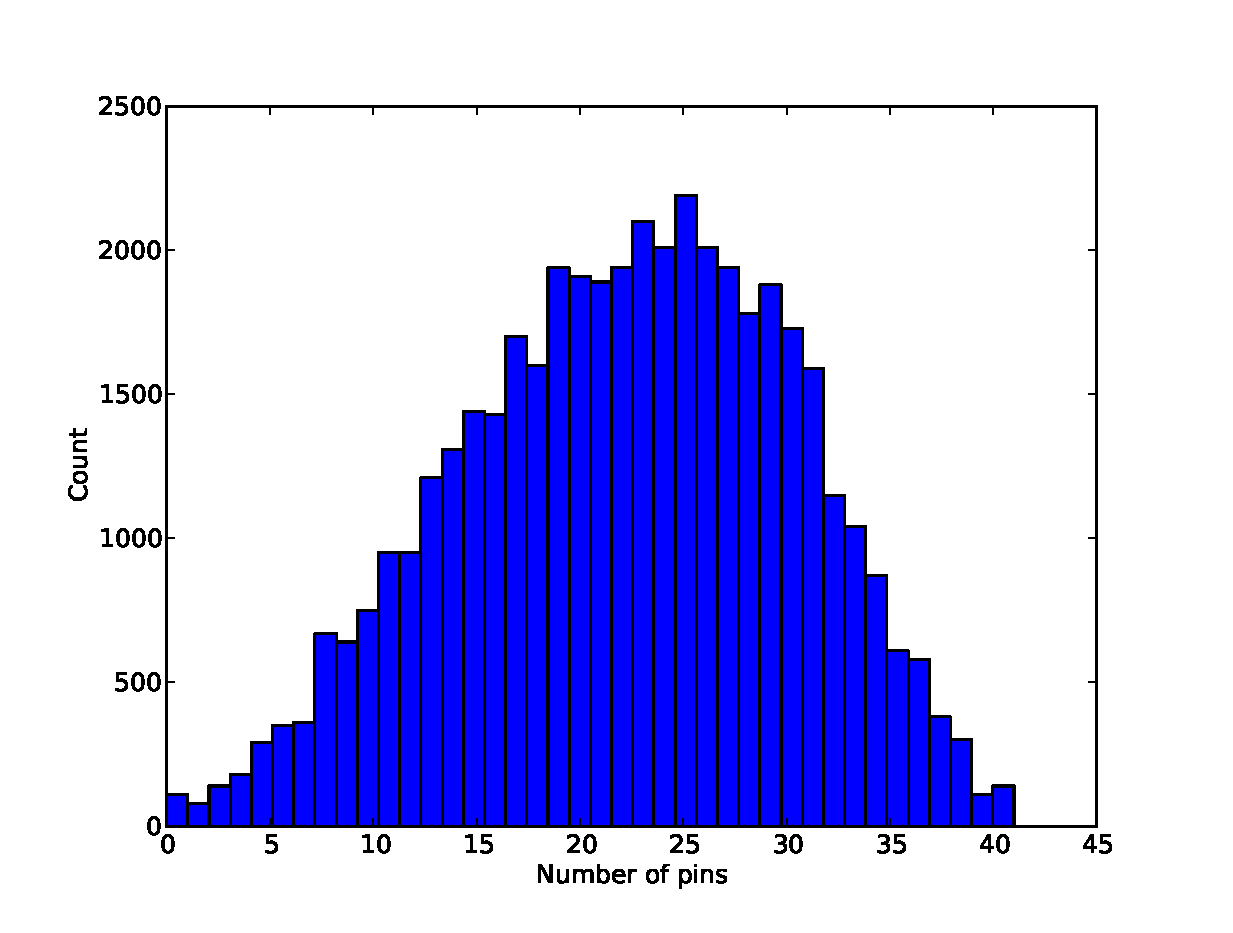
\includegraphics[width=\textwidth]{Images/complexity_hist.eps}
\caption{Histogram of the complexity the $4425$ schematics used for evaluation.}
\label{fig:complexity_hist}
\end{center}
\end{figure}

To compare success rates, we will look at number of successes out of $10$ runs
on each of the $4425$ schematics. To compare running time, we will look at CPU
time spent on the wiring step, as the placement step has much less variability.
To compare the goodness of layouts, we will look at numbers of wires, total
lengths of wires, numbers of wire crosses, and our layout badness metric as
functions of circuit complexity. Note that in all figures that follow,
error bars indicate $1.96$ times the standard error. For each comparison,
we present exemplar layouts generated by the alternative methods for the
schematic shown in Figure \ref{fig:exemplar_schematic}.

\begin{figure}
\begin{center}
\includegraphics[width=\textwidth]{Images/exemplar_schematic.png}
\caption{Exemplar schematic.}
\label{fig:exemplar_schematic}
\end{center}
\end{figure}

\section{Comparing Placement Methods}
\label{sec:compare_placement}

\begin{figure}[H]
\begin{center}
\includegraphics[width=\textwidth]{Images/exemplar_per_pair_decreasing.png}
\caption{Blocking exemplar.}
\end{center}
\end{figure}

\begin{figure}[H]
\begin{center}
\includegraphics[width=\textwidth]{Images/exemplar_distance.png}
\caption{Distance exemplar.}
\end{center}
\end{figure}

\begin{figure}[H]
\begin{center}
\includegraphics[width=\textwidth]{Images/placement_success_comparison.eps}
\caption{Placement method comparison: success rates.}
\label{fig:placement_success}
\end{center}
\end{figure}

\begin{table}[H]
\begin{center}
\begin{singlespace}
\begin{tabular}{|c||c|c|c|c|c|c|c|c|c|c|c|}
\hline
 & \multicolumn{11}{|c|}{Number of times succeeded out of $10$} \\
\hline
 & 0 & 1 & 2 & 3 & 4 & 5 & 6 & 7 & 8 & 9 & 10 \\
\hline\hline
Blocking & $162$ & $38$ & $51$ & $57$ & $72$ & $85$ & $109$ & $106$ & $144$ & $203$ & $3398$ \\
 & $0.04$ & $0.01$ & $0.01$ & $0.01$ & $0.02$ & $0.02$ & $0.02$ & $0.02$ & $0.03$ & $0.05$ & $0.77$ \\
\hline
 Distance & $258$ & $55$ & $54$ & $50$ & $52$ & $77$ & $86$ & $97$ & $93$ & $130$ & $3473$ \\
  & $0.06$ & $0.01$ & $0.01$ & $0.01$ & $0.01$ & $0.02$ & $0.02$ & $0.02$ & $0.02$ & $0.03$ & $0.78$ \\
\hline
  Random & $893$ & $512$ & $387$ & $364$ & $292$ & $259$ & $247$ & $277$ & $311$ & $321$ & $562$ \\
   & $0.20$ & $0.12$ & $0.09$ & $0.08$ & $0.07$ & $0.06$ & $0.06$ & $0.06$ & $0.07$ & $0.07$ & $0.13$ \\
\hline
\end{tabular}
\end{singlespace}
\end{center}
\label{tb:placement_success}
\caption{Placement method comparison: success rates.}
\end{table}

\begin{figure}[H]
\begin{center}
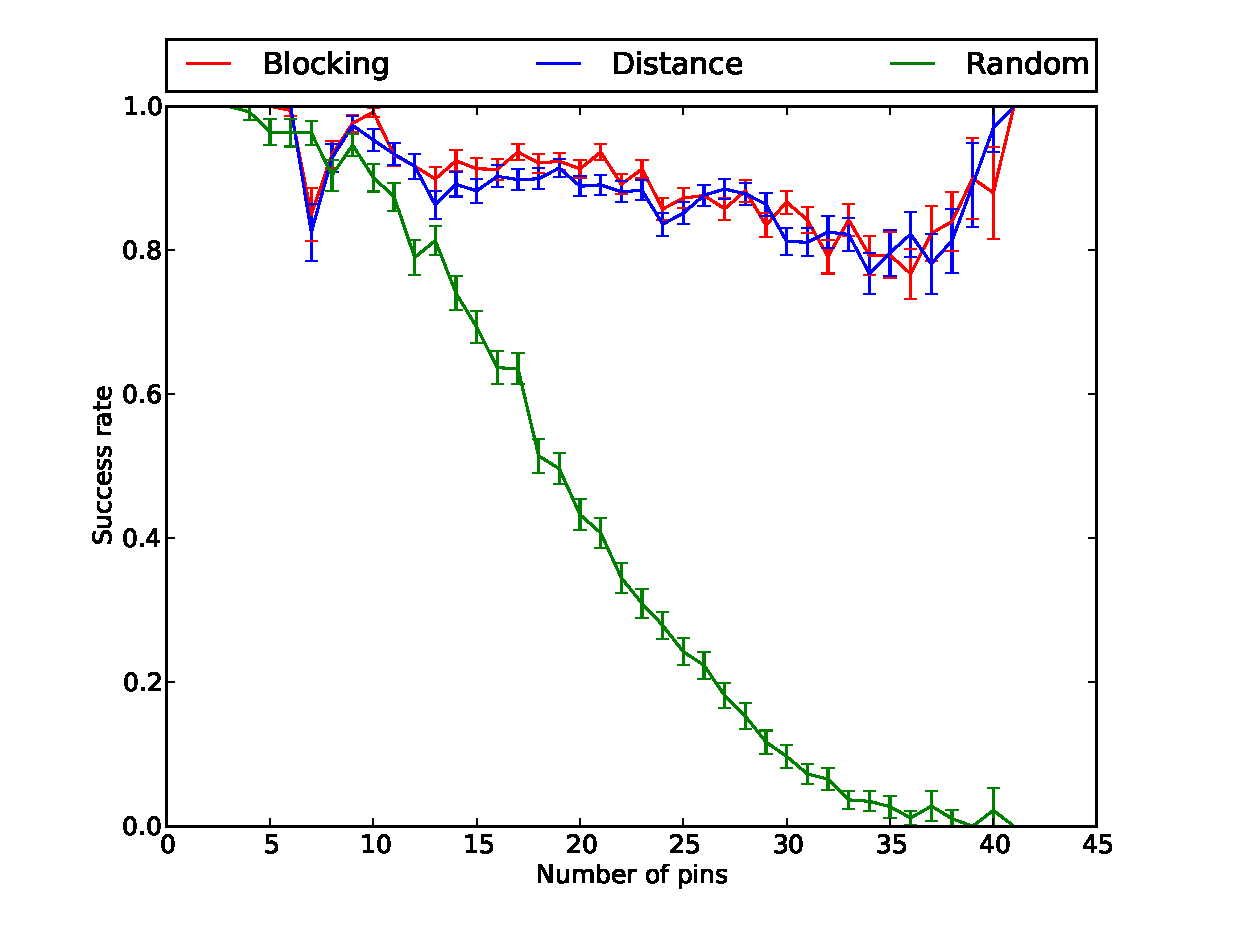
\includegraphics[width=\textwidth]{Images/placement_success_trend_comparison.eps}
\caption{Placement method comparison: success rate trends.}
\label{fig:placement_success_trend}
\end{center}
\end{figure}

\begin{figure}[H]
\begin{center}
\includegraphics[width=\textwidth]{Images/placement_time_trend_comparison.eps}
\caption{Placement method comparison: wiring time trends.}
\label{fig:placement_time_trend}
\end{center}
\end{figure}

\begin{figure}
\begin{center}
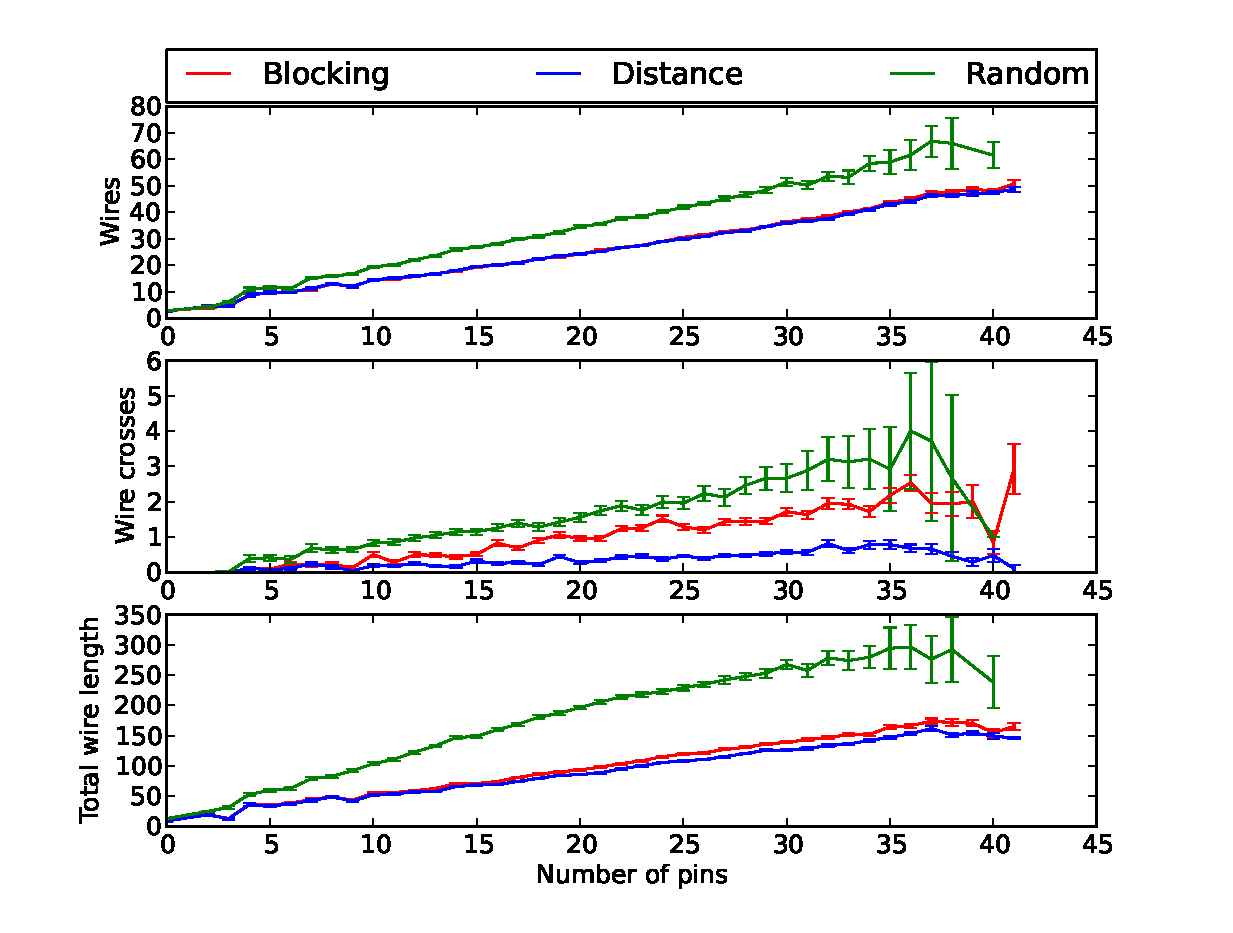
\includegraphics[width=\textwidth]{Images/placement_quality_trend_comparison.eps}
\caption{Placement method comparison: layout quality trends.}
\label{fig:placement_quality_trend}
\end{center}
\end{figure}

\begin{figure}
\begin{center}
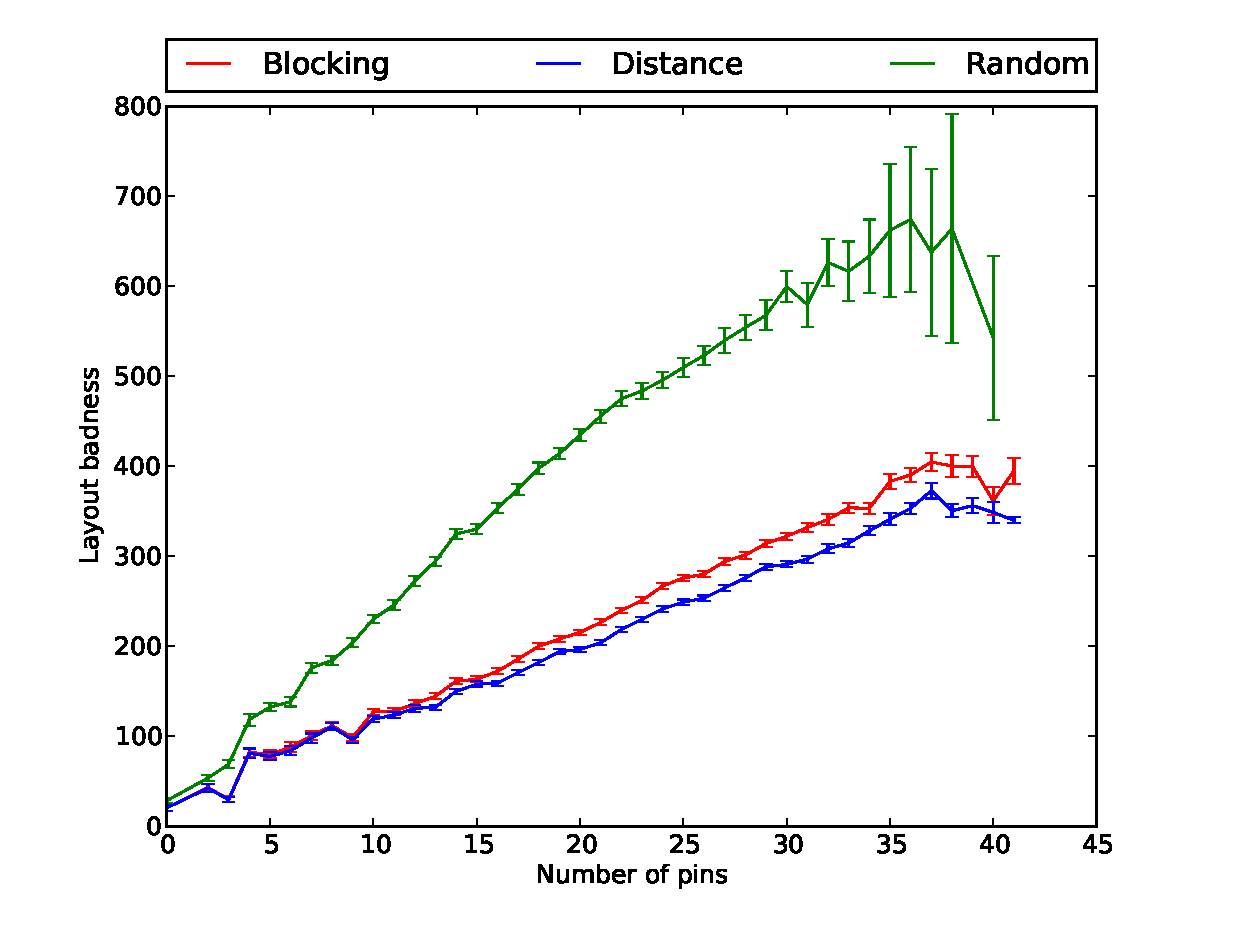
\includegraphics[width=\textwidth]{Images/placement_badness_trend_comparison.eps}
\caption{Placement method comparison: layout badness trends.}
\label{fig:placement_badness_trend}
\end{center}
\end{figure}

\section{Comparing Wiring Methods}

\begin{figure}[H]
\begin{center}
\includegraphics[width=\textwidth]{Images/exemplar_all_pairs.png}
\caption{All pairs exemplar.}
\end{center}
\end{figure}

\begin{figure}[H]
\begin{center}
\includegraphics[width=\textwidth]{Images/exemplar_per_node_increasing.png}
\caption{Per-node, increasing exemplar.}
\end{center}
\end{figure}

\begin{figure}[H]
\begin{center}
\includegraphics[width=\textwidth]{Images/exemplar_per_node_decreasing.png}
\caption{Per-node, decreasing exemplar.
We used the distance based placement method instead of the blocking based
placement method to generate this exemplar as the
combination of the blocking based method with this wiring method consistently
failed on the schematic shown in Figure \ref{fig:exemplar_schematic}.}
\end{center}
\end{figure}

\begin{figure}[H]
\begin{center}
\includegraphics[width=\textwidth]{Images/exemplar_per_pair_increasing.png}
\caption{Per-pair, increasing exemplar.}
\end{center}
\end{figure}

\begin{figure}[H]
\begin{center}
\includegraphics[width=\textwidth]{Images/exemplar_per_pair_decreasing.png}
\caption{Per-pair, decreasing exemplar.}
\end{center}
\end{figure}

\begin{figure}[H]
\begin{center}
\includegraphics[width=\textwidth]{Images/exemplar_straight_wiring.png}
\caption{Straight wiring exemplar.}
\end{center}
\end{figure}

\begin{figure}[H]
\begin{center}
\includegraphics[width=\textwidth]{Images/wiring_success_comparison.eps}
\caption{Wiring method comparison: success rates.}
\label{fig:wiring_success}
\end{center}
\end{figure}

\begin{table}[H]
\begin{center}
\begin{singlespace}
\begin{tabular}{|c||c|c|c|c|c|c|c|c|c|c|c|}
\hline
 & \multicolumn{11}{|c|}{Number of times succeeded out of $10$} \\
\hline
 & 0 & 1 & 2 & 3 & 4 & 5 & 6 & 7 & 8 & 9 & 10 \\
\hline\hline
All & $458$ & $114$ & $111$ & $112$ & $127$ & $145$ & $177$ & $139$ & $172$ & $227$ & $2643$ \\
 & $0.10$ & $0.03$ & $0.03$ & $0.03$ & $0.03$ & $0.03$ & $0.04$ & $0.03$ & $0.04$ & $0.05$ & $0.60$ \\
\hline
 Node I & $154$ & $50$ & $55$ & $62$ & $85$ & $71$ & $106$ & $141$ & $156$ & $217$ & $3328$ \\
  & $0.03$ & $0.01$ & $0.01$ & $0.01$ & $0.02$ & $0.02$ & $0.02$ & $0.03$ & $0.04$ & $0.05$ & $0.75$ \\
\hline
  Node D & $195$ & $50$ & $58$ & $66$ & $104$ & $83$ & $125$ & $176$ & $162$ & $268$ & $3138$ \\
   & $0.04$ & $0.01$ & $0.01$ & $0.01$ & $0.02$ & $0.02$ & $0.03$ & $0.04$ & $0.04$ & $0.06$ & $0.71$ \\
\hline
   Pair I & $177$ & $40$ & $59$ & $54$ & $91$ & $92$ & $100$ & $118$ & $132$ & $212$ & $3350$ \\
    & $0.04$ & $0.01$ & $0.01$ & $0.01$ & $0.02$ & $0.02$ & $0.02$ & $0.03$ & $0.03$ & $0.05$ & $0.76$ \\
\hline
    Pair D & $162$ & $38$ & $51$ & $57$ & $72$ & $85$ & $109$ & $106$ & $144$ & $203$ & $3398$ \\
     & $0.04$ & $0.01$ & $0.01$ & $0.01$ & $0.02$ & $0.02$ & $0.02$ & $0.02$ & $0.03$ & $0.05$ & $0.77$ \\
\hline
     Straight & $0$ & $0$ & $0$ & $0$ & $0$ & $0$ & $0$ & $0$ & $0$ & $0$ & $4425$ \\
      & $0.00$ & $0.00$ & $0.00$ & $0.00$ & $0.00$ & $0.00$ & $0.00$ & $0.00$ & $0.00$ & $0.00$ & $1.00$ \\
\hline
\end{tabular}
\end{singlespace}
\end{center}
\label{tb:wiring_success}
\caption{Wiring method comparison: success rates.}
\end{table}

\begin{figure}[H]
\centering
\subfigure[All pairs]{
\includegraphics[width=7cm]{Images/wiring_all_success_trend.eps}}
\subfigure[Per-node]{
\includegraphics[width=7cm]{Images/wiring_node_success_trend.eps}}
\subfigure[Per-pair]{
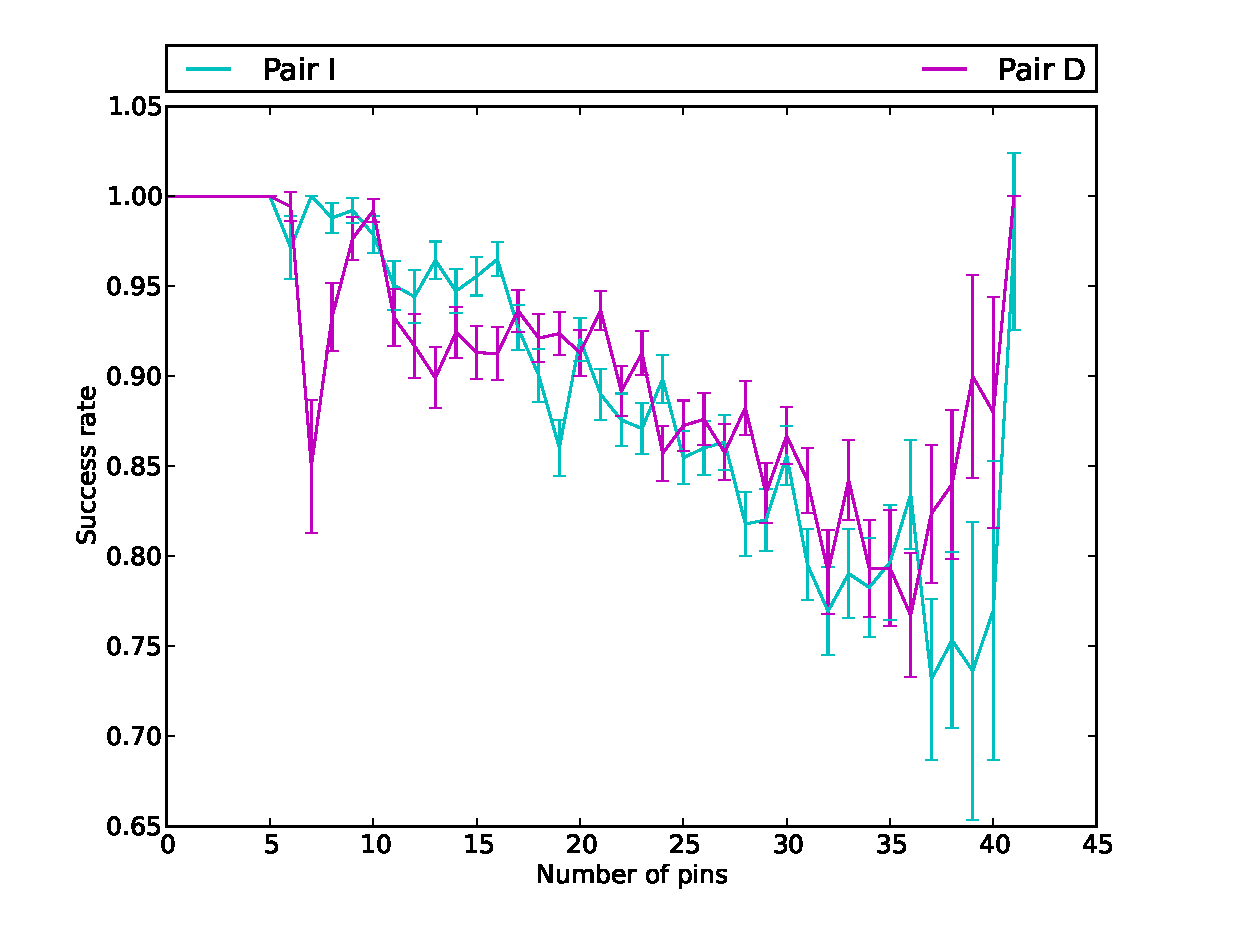
\includegraphics[width=7cm]{Images/wiring_pair_success_trend.eps}}
\label{fig:wiring_success_trend}
\caption{Wiring method comparison: success rate trends.}
\end{figure}

\begin{figure}[H]
\begin{center}
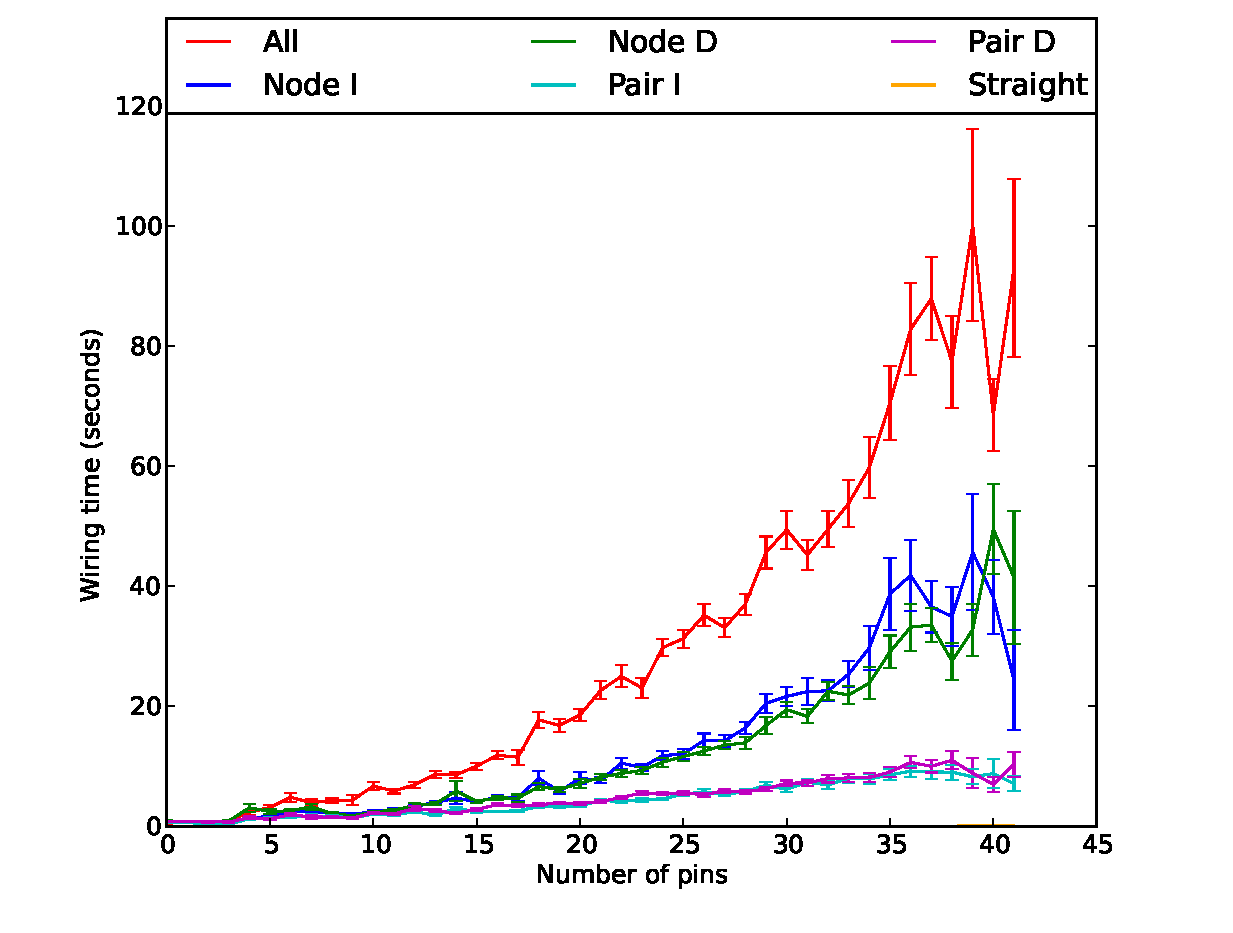
\includegraphics[width=\textwidth]{Images/wiring_time_trend_comparison.eps}
\caption{Wiring method comparison: wiring time trends.}
\label{fig:wiring_time_trend}
\end{center}
\end{figure}

\begin{figure}[H]
\begin{center}
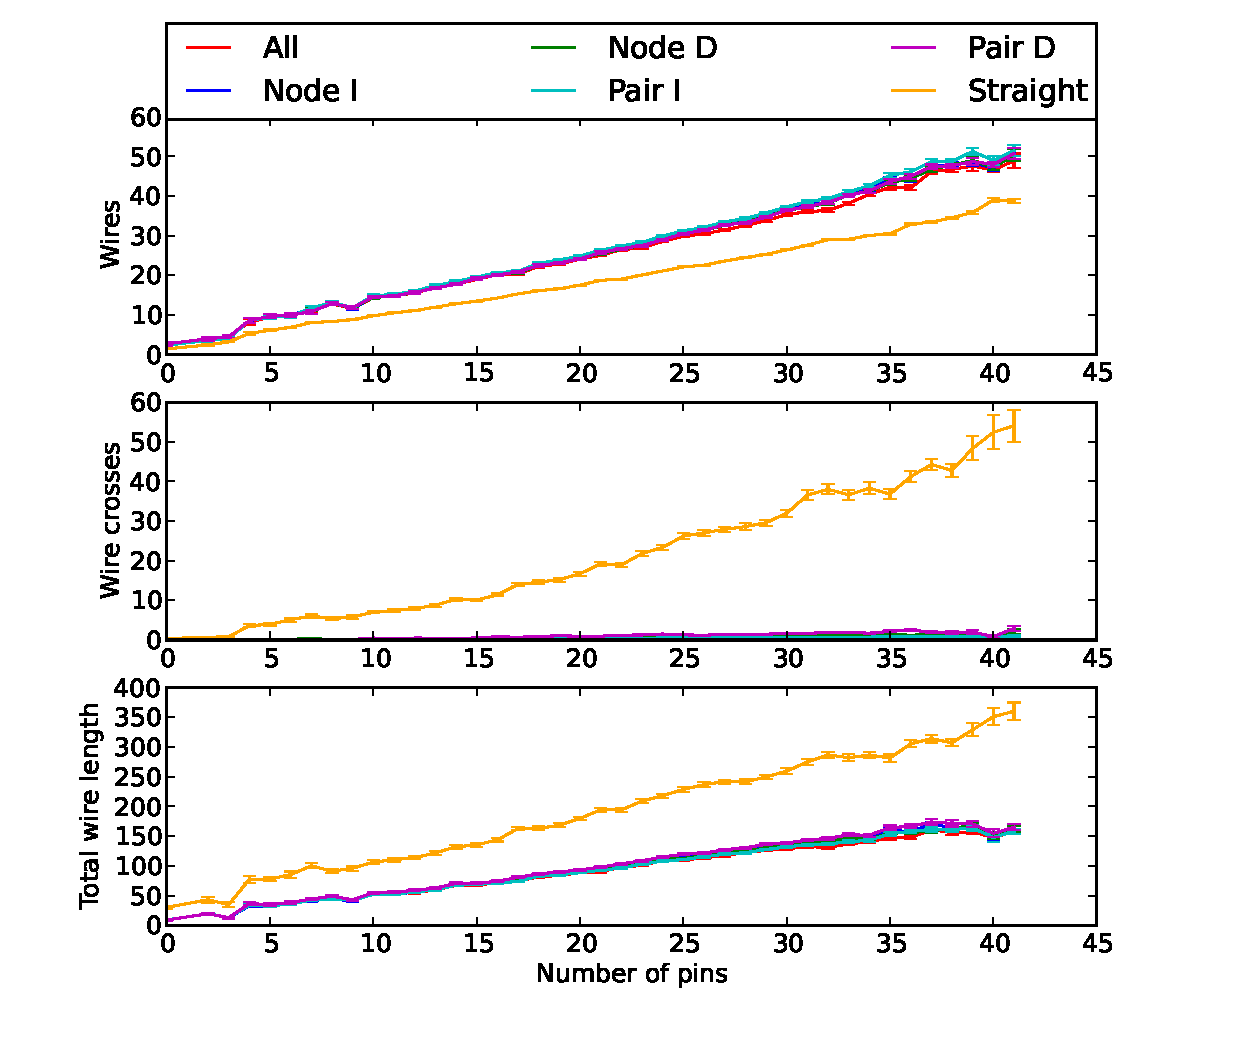
\includegraphics[width=\textwidth]{Images/wiring_quality_trend_comparison.eps}
\caption{Wiring method comparison: layout quality trends.}
\label{fig:wiring_quality_trend}
\end{center}
\end{figure}

\begin{figure}[H]
\begin{center}
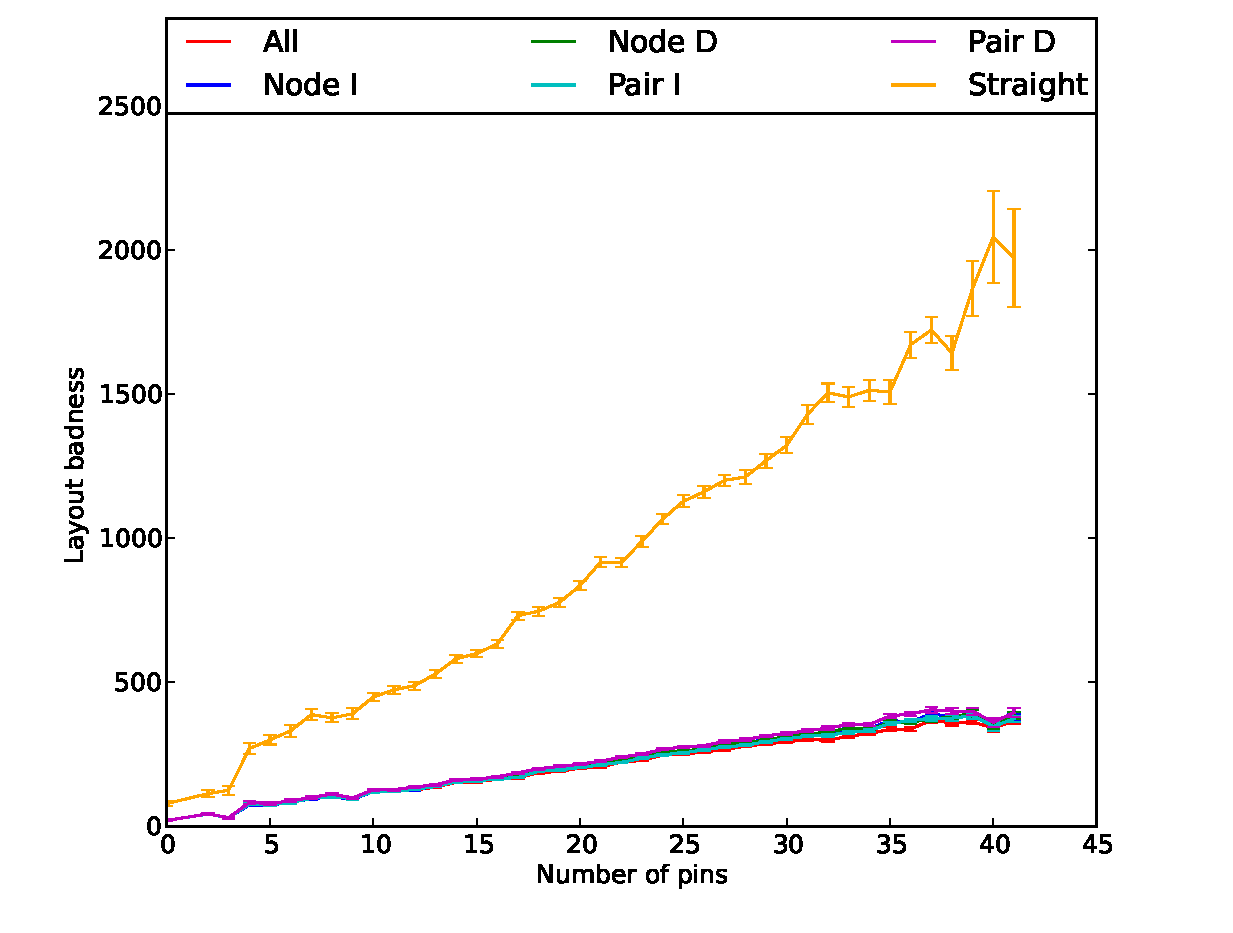
\includegraphics[width=\textwidth]{Images/wiring_badness_trend_comparison.eps}
\caption{Wiring method comparison: layout badness trends.}
\label{fig:wiring_badness_trend}
\end{center}
\end{figure}

\section{Effect of limiting the number of vertices to expand in $A*$}
\label{sec:expand_limit}

For each of the $5$ wiring methods we have looked at, we have run tests on $4425$
schematics. We have tested each method $10$ times on each schematic. Hench, we
have $44250$ data points for each of the wiring methods. Here we provide
histograms that show the maximum number of expanded vertices in the $A*$ search
among the $44250$ runs for each of the $5$ methods.

\begin{figure}[H]
\begin{center}
\includegraphics[width=\textwidth]{Images/max_expanded_all_pairs.eps}
\caption{Histogram of number of vertices expanded for all pairs wiring.}
\label{fig:max_expanded_all_pairs}
\end{center}
\end{figure}

\begin{figure}[H]
\begin{center}
\includegraphics[width=\textwidth]{Images/max_expanded_per_node_increasing.eps}
\caption{Histogram of maximum number of vertices expanded for per-node,
increasing wiring.}
\label{fig:max_expanded_per_node_increasing}
\end{center}
\end{figure}

\begin{figure}[H]
\begin{center}
\includegraphics[width=\textwidth]{Images/max_expanded_per_node_decreasing.eps}
\caption{Histogram of maximum number of vertices expanded for per-node,
decreasing wiring.}
\label{fig:max_expanded_per_node_decreasing}
\end{center}
\end{figure}

\begin{figure}[H]
\begin{center}
\includegraphics[width=\textwidth]{Images/max_expanded_per_pair_increasing.eps}
\caption{Histogram of maximum number of vertices expanded for per-pair,
increasing wiring.}
\label{fig:max_expanded_per_pair_increasing}
\end{center}
\end{figure}

\begin{figure}[H]
\begin{center}
\includegraphics[width=\textwidth]{Images/max_expanded_per_pair_decreasing.eps}
\caption{Histogram of maximum number of vertices expanded for per-pair,
decreasing wiring.}
\label{fig:max_expanded_per_pair_decreasing}
\end{center}
\end{figure}

\section{Comparing Search Methods}

\begin{figure}[H]
\begin{center}
\includegraphics[width=\textwidth]{Images/exemplar_per_pair_decreasing.png}
\caption{$A*$ Search exemplar.}
\end{center}
\end{figure}

\begin{figure}[H]
\begin{center}
\includegraphics[width=\textwidth]{Images/exemplar_best_first.png}
\caption{Best First Search exemplar.}
\end{center}
\end{figure}

\begin{figure}[H]
\begin{center}
\includegraphics[width=\textwidth]{Images/search_success_comparison.eps}
\caption{Search method comparison: success rates.}
\label{fig:search_success}
\end{center}
\end{figure}

\begin{table}[H]
\begin{center}
\begin{singlespace}
\begin{tabular}{|c||c|c|c|c|c|c|c|c|c|c|c|}
\hline
 & \multicolumn{11}{|c|}{Number of times succeeded out of $10$} \\
\hline
 & 0 & 1 & 2 & 3 & 4 & 5 & 6 & 7 & 8 & 9 & 10 \\
\hline\hline
$A*$ & $162$ & $38$ & $51$ & $57$ & $72$ & $85$ & $109$ & $106$ & $144$ & $203$ & $3398$ \\
 & $0.04$ & $0.01$ & $0.01$ & $0.01$ & $0.02$ & $0.02$ & $0.02$ & $0.02$ & $0.03$ & $0.05$ & $0.77$ \\
\hline
 Best First & $6$ & $5$ & $2$ & $1$ & $13$ & $10$ & $29$ & $45$ & $84$ & $245$ & $3985$ \\
  & $0.00$ & $0.00$ & $0.00$ & $0.00$ & $0.00$ & $0.00$ & $0.01$ & $0.01$ & $0.02$ & $0.06$ & $0.90$ \\
\hline
\end{tabular}
\end{singlespace}
\end{center}
\label{tb:search_success}
\caption{Search method comparison: success rates.}
\end{table}

\begin{figure}[H]
\begin{center}
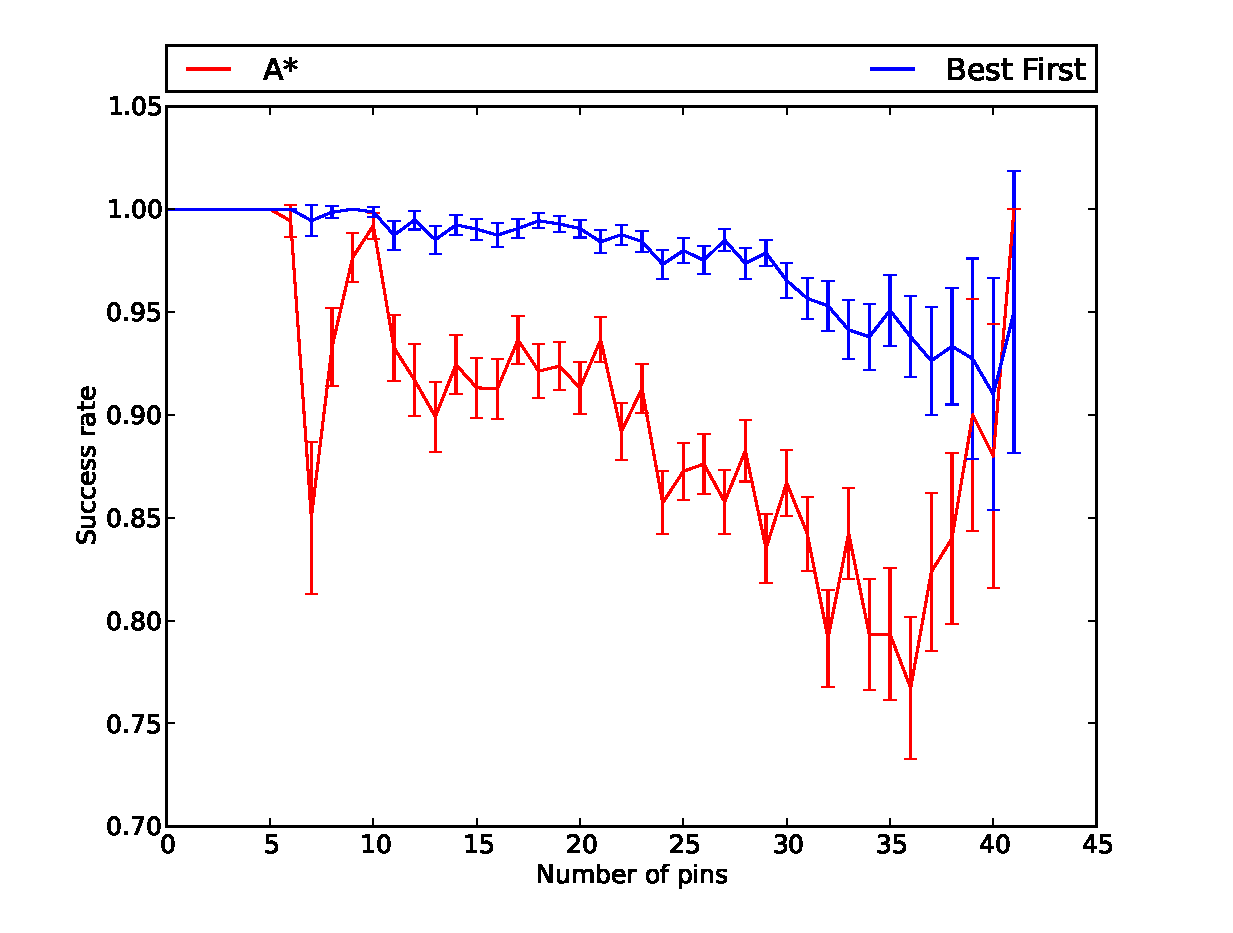
\includegraphics[width=\textwidth]{Images/search_success_trend_comparison.eps}
\caption{Search method comparison: success rate trends.}
\label{fig:search_success_trend}
\end{center}
\end{figure}

\begin{figure}[H]
\begin{center}
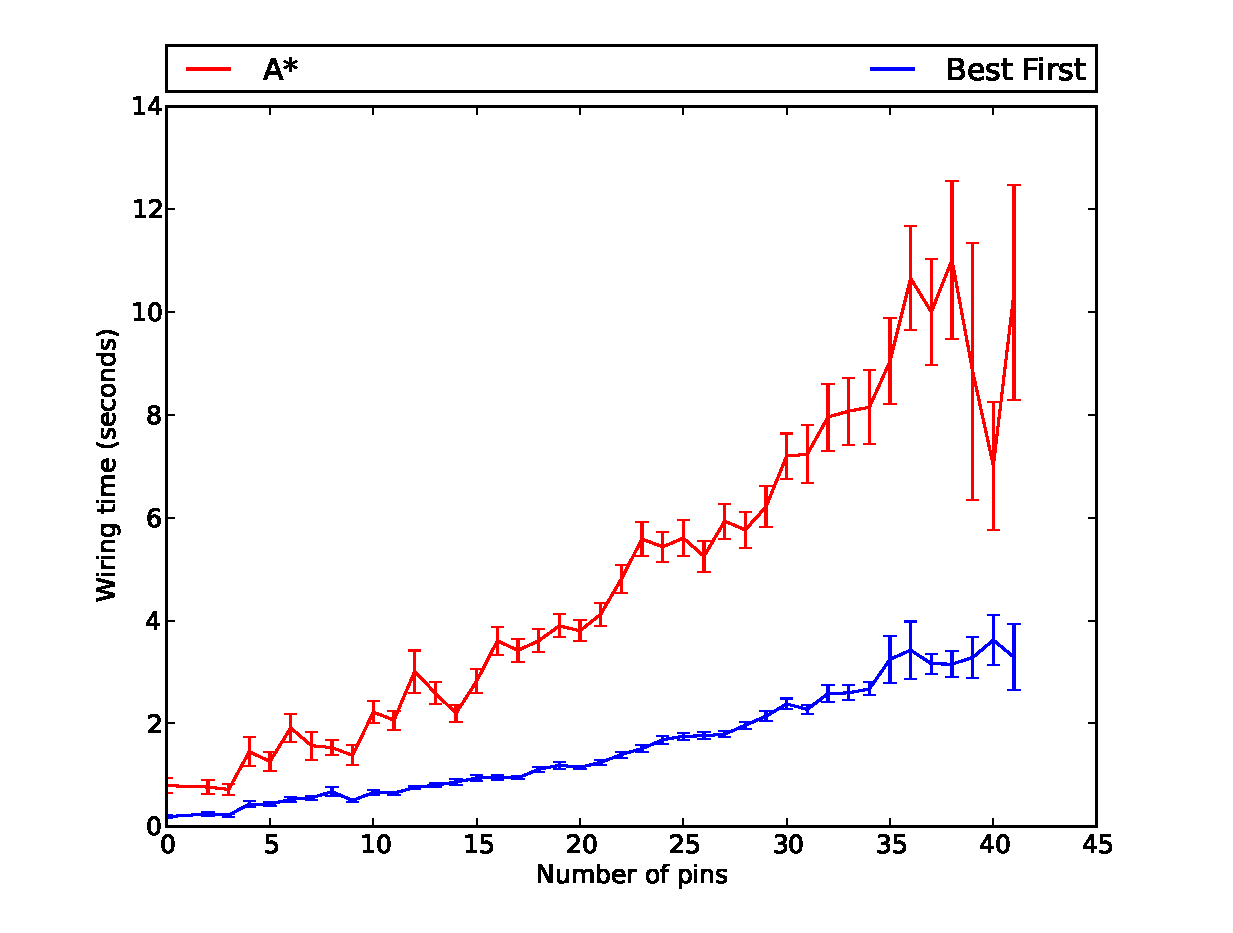
\includegraphics[width=\textwidth]{Images/search_time_trend_comparison.eps}
\caption{Search method comparison: wiring time trends.}
\label{fig:search_time_trend}
\end{center}
\end{figure}

\begin{figure}[H]
\begin{center}
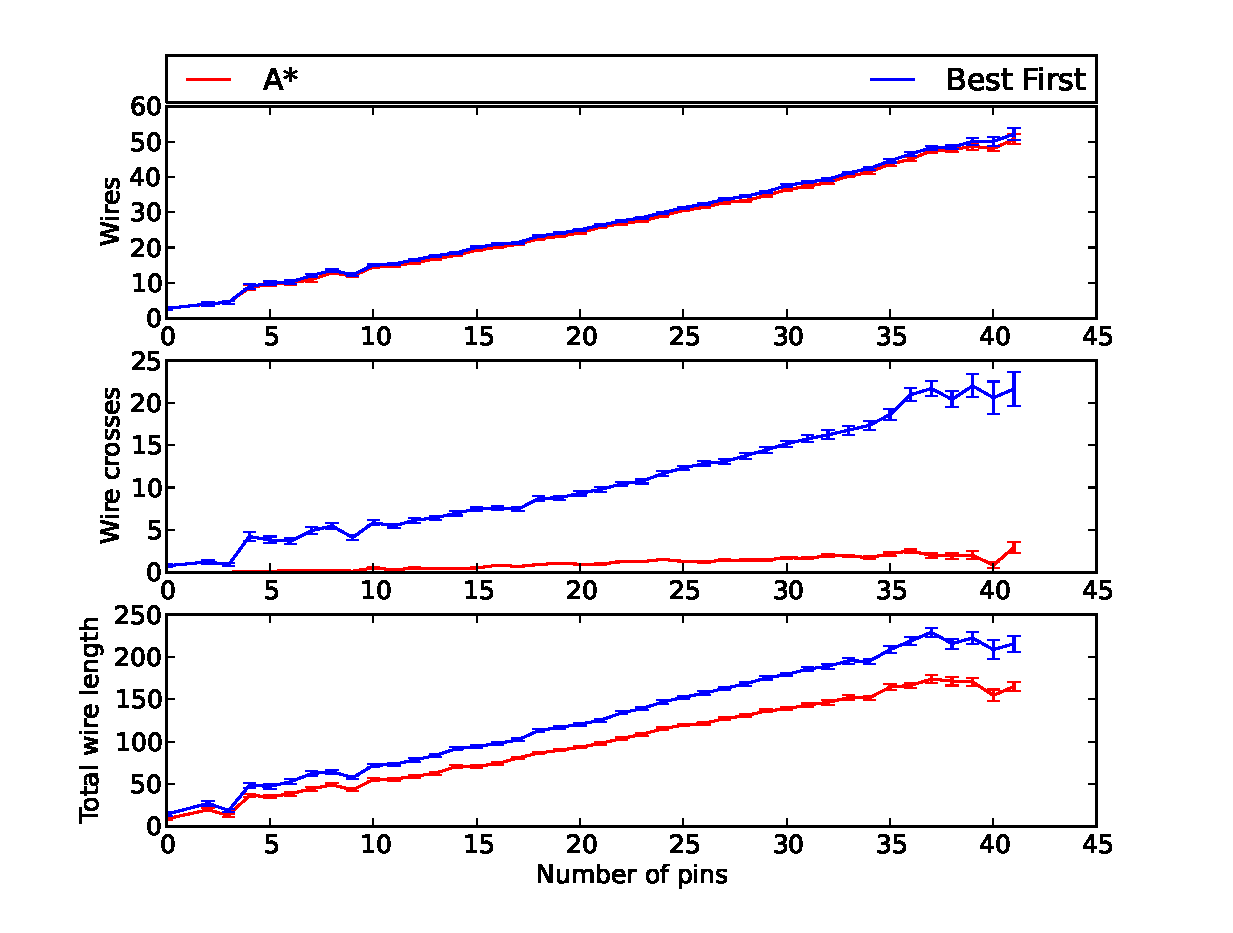
\includegraphics[width=\textwidth]{Images/search_quality_trend_comparison.eps}
\caption{Search method comparison: layout quality trends.}
\label{fig:search_quality_trend}
\end{center}
\end{figure}

\begin{figure}[H]
\begin{center}
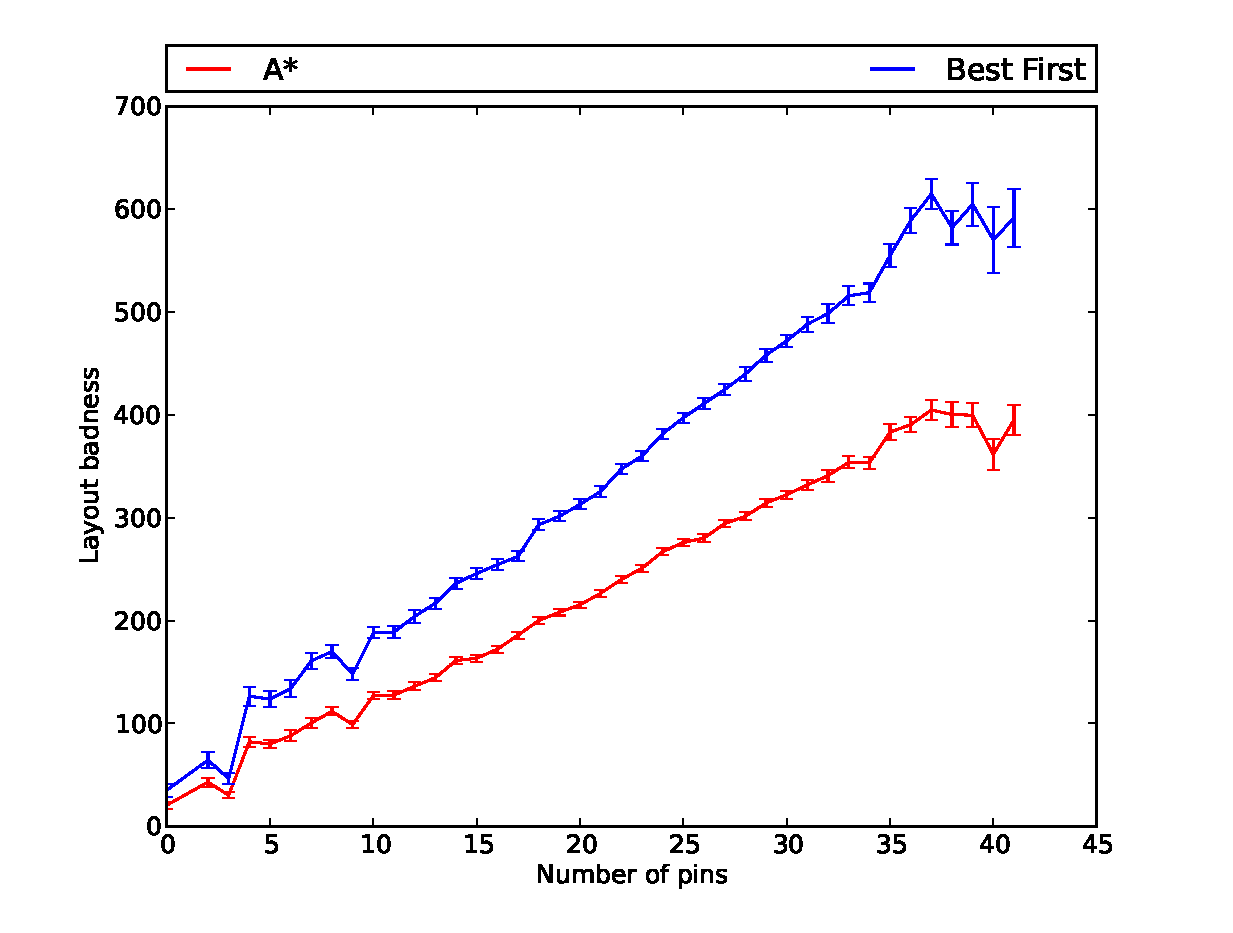
\includegraphics[width=\textwidth]{Images/search_badness_trend_comparison.eps}
\caption{Search method comparison: layout badness trends.}
\label{fig:search_badness_trend}
\end{center}
\end{figure}

\section{Combined Algorithm}
\label{sec:combined_algorithm}

Here we provide data for the combined algorithm presented in Section
\ref{sec:combined_alg}. To generate this data, we used a different dataset of
$4425$ schematics. As desired, the algorithm has a $100\%$ success rate.
Figure \ref{fig:final_num_trials} gives a breakdown of how the algorithm
succeeded. The first four columns correspond to success from one of the four
combinations of placement and wiring methods. The last 5 columns correspond to
layouts in which none of the four combinations was successful on all pairs of
locations and we had to connect a few pairs of locations by putting down a
straight wire bridging the locations. Figure
\ref{fig:final_time_trend} gives the average total time taken by the algorithm
as a function of circuit complexity. Finally, Figures
\ref{fig:final_quality_trend} and \ref{fig:final_badness_trend}
give statistics on the quality of the layouts produced by the combined algorithm
as a function of circuit complexity.

\begin{figure}[H]
\begin{center}
\includegraphics[width=\textwidth]{Images/exemplar_combined_algorithm.png}
\caption{Combined algorithm exemplar.}
\end{center}
\end{figure}

\begin{figure}[H]
\begin{center}
\includegraphics[width=\textwidth]{Images/final_algorithm_num_trials.eps}
\caption{Combined algorithm success summary.}
\label{fig:final_num_trials}
\end{center}
\end{figure}

\begin{figure}[H]
\begin{center}
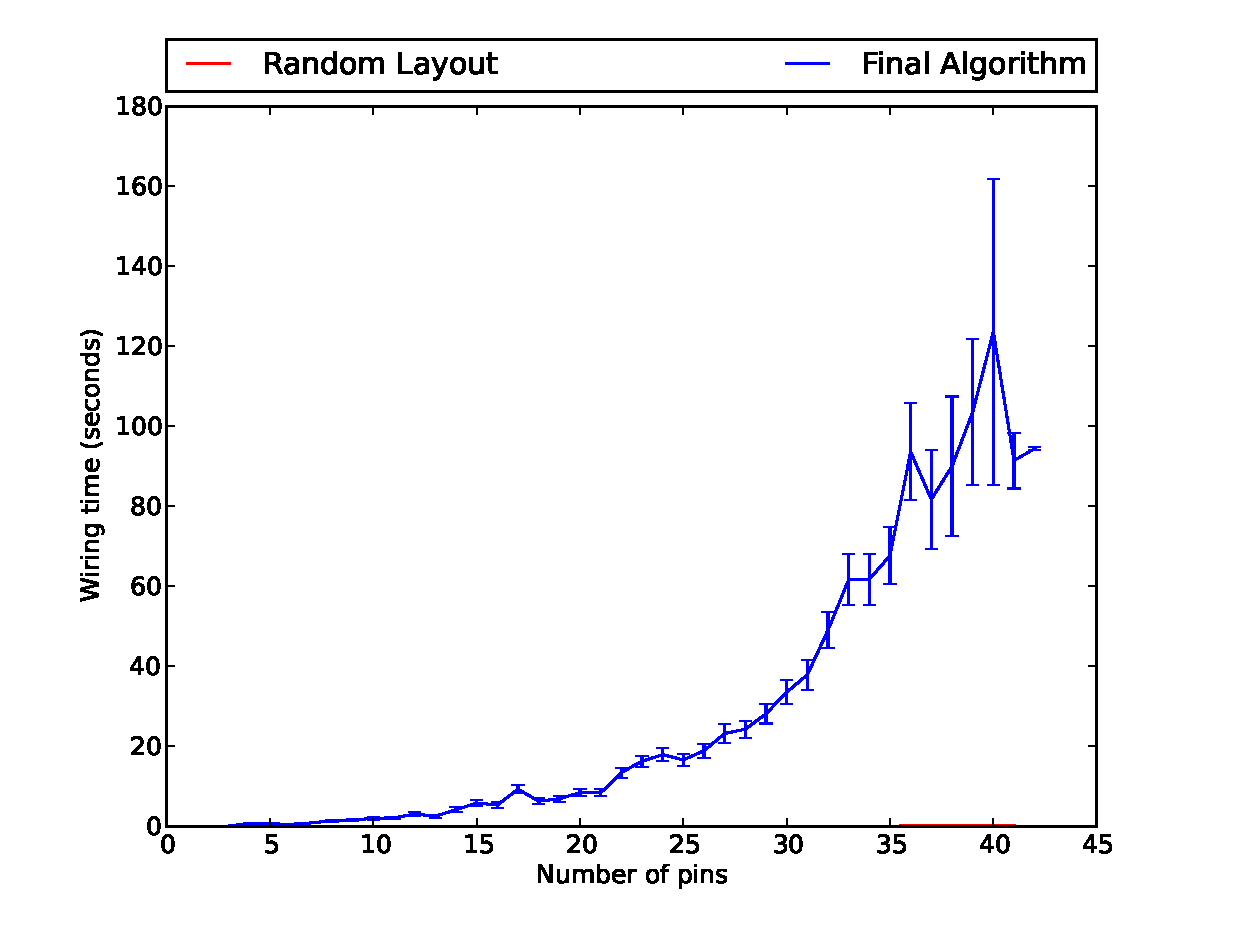
\includegraphics[width=\textwidth]{Images/final_algorithm_time_trend.eps}
\caption{Combined algorithm total CPU time trend as a function of circuit
complexity.}
\label{fig:final_time_trend}
\end{center}
\end{figure}

\begin{figure}[H]
\begin{center}
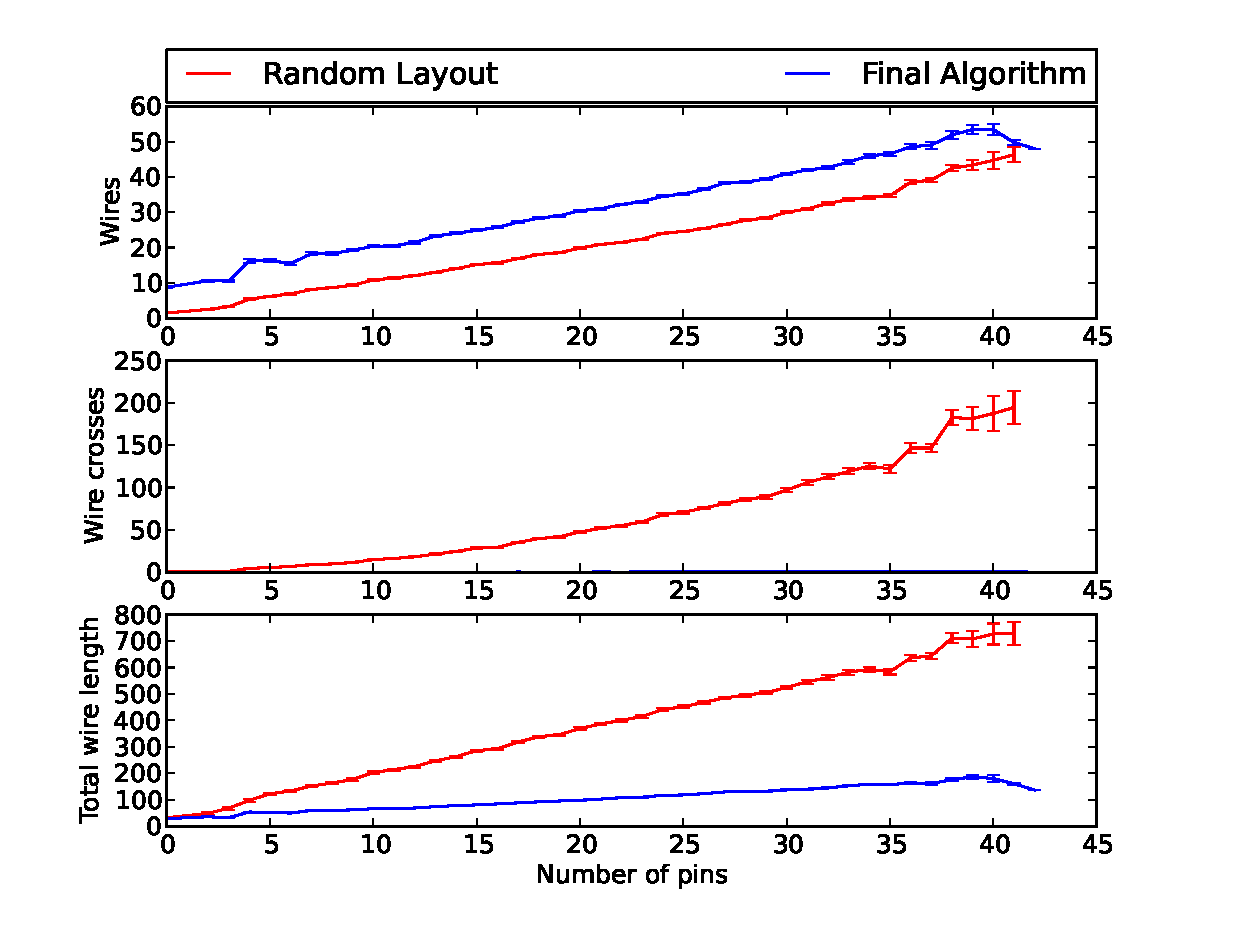
\includegraphics[width=\textwidth]{Images/final_algorithm_quality_trend.eps}
\caption{Combined algorithm quality trend.}
\label{fig:final_quality_trend}
\end{center}
\end{figure}

\begin{figure}[H]
\begin{center}
\includegraphics[width=\textwidth]{Images/final_algorithm_badness_trend.eps}
\caption{Combined algorithm layout badness trend.}
\label{fig:final_badness_trend}
\end{center}
\end{figure}
